\documentclass[border=10pt]{standalone}
\usepackage{pgfplots}
\pgfplotsset{compat=1.18}
\begin{document}
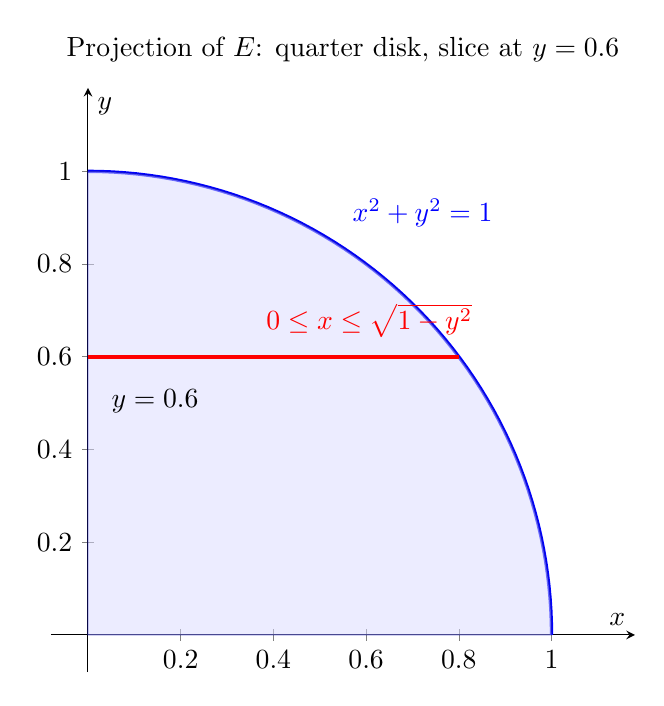
\begin{tikzpicture}
\begin{axis}[
    axis lines=middle,
    xlabel={$x$}, ylabel={$y$},
    title={Projection of $E$: quarter disk, slice at $y=0.6$},
    xmin=-0.08, xmax=1.18, ymin=-0.08, ymax=1.18,
    width=9cm, height=9cm,
    axis equal image,
    domain=0:90, samples=60,
]
% quarter disk boundary
\addplot[blue, very thick] ({cos(x)},{sin(x)});
\addplot[blue!70!black, fill=blue!15, opacity=0.5] ({cos(x)},{sin(x)}) \closedcycle;
% vertical slice at y = 0.6 : x from 0 to sqrt(1-y^2)
\addplot[red, ultra thick] coordinates {(0,0.6) ({sqrt(1-0.36)},0.6)};
\node[red, anchor=south east] at (axis cs:0.85,0.62) {$0\le x\le\sqrt{1-y^2}$};
\node[blue, anchor=south west] at (axis cs:0.55,0.86) {$x^2+y^2=1$};
\node[anchor=north west] at (axis cs:0.03,0.55) {$y=0.6$};
\end{axis}
\end{tikzpicture}
\end{document}
